A Ecofont possui design baseado na velha fonte Vera Sans. Por�m, ela tem um diferencial: pequenos buraquinhos circulares congruentes, e em todo o seu corpo, presentes em cada s�mbolo. Esses furos proporcionam um gasto de tinta menor na hora da impress�o. 

\begin{figure}[h]
\centering
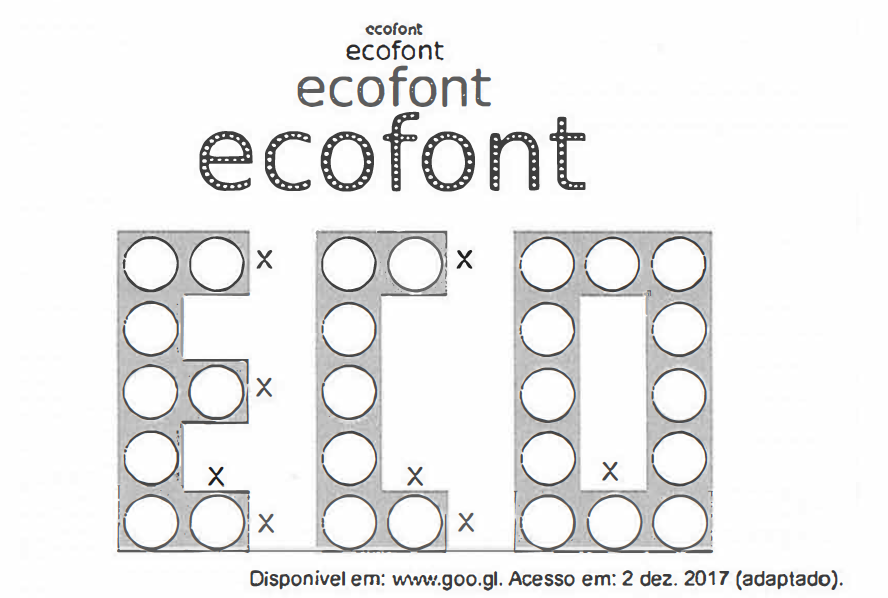
\includegraphics[width=8cm]{../figuras/q156-2018}
\end{figure}

Suponha que a palavra ECO esteja escrita nessa fonte, com tamanho 192, e que seja composta por letras formadas por quadrados de lados x com furos circulares de raio $r=\frac x 3$. 
Para que a �rea a ser pintada seja reduzida a $\frac 1 16$ da �rea inicial, pretende-se reduzir o tamanho da fonte. Sabe-se que, ao alterar o tamanho da fonte, o tamanho da letra � alterado na mesma propor��o. Nessas condi��es, o tamanho adequado da fonte ser� 

\begin{enumerate}
\item[a)]64
\item[b)]48
\item[c)]24
\item[d)]21
\item[e)]12
\end{enumerate}